\asection{Experiment Results}
\label{Experiment Results}
This section presents the results of the experiments described in Chapter \ref{Description Conducted Experiments}.An evaluation of the results is
performed before the algorithms can be compared against each other based on the criteria specified in chapter \ref{The comparison criteria}, namely the time and 
space efficiency of the algorithms.

\subsection{Joined graph results for the evaluation of different vertice numbers experiment}
This section presents the time and memory results for experiment described in section \ref{Performance evaluation for different vertice numbers}. The 
experiment is conducted on joined graphs.
\subsubsection{Memory Results}
\label{Memory Results}
This section compares the efficiency of the two algorithms in terms of their memory. The amount of virtual memory used by the two algorithms are graphically 
represented, analysed and a conclusion of as to which of the two algorithm is more efficient in terms of memory is reached based on figure \ref{fig:memory_comparison}.
The red line depics the amount of memory used by the Ullman algorithm and the blue line depicts the amount of memory used by the VF2 algorithm.
\begin{figure}[H]
  \begin{center}
      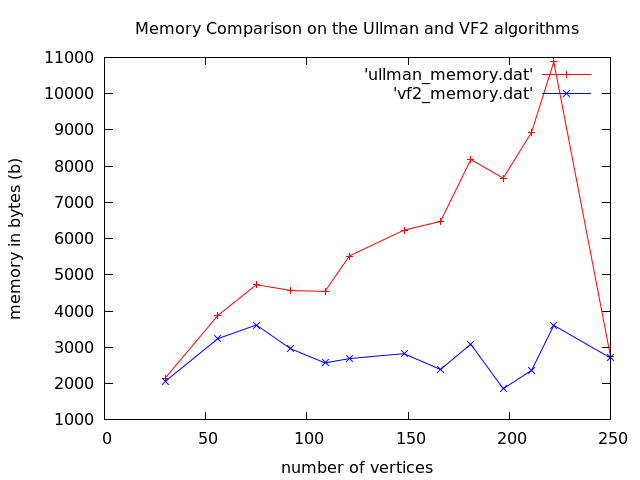
\includegraphics[width=0.8\textwidth]{memory_comparison.png}
  \end{center}    
  \caption{Graph depiting the results for the memory comparison between the algorithms for joined graphs}
  \label{fig:memory_comparison}
\end{figure}

\paragraph{Analysis of results}\mbox{}\\
Figure \ref{fig:memory_comparison} depicts the comparison of the Ullman and the VF2 algorithms on the criteria of memory used during the execution of the graph matching processes
of the respective algorithms.\newline\newline
The virtual memory used by the the Ullman algorithm is depicted by the \textit{red} line in figure \ref{fig:memory_comparison} and the \textit{blue} line
represents the virtual memory used by the VF2 algorithm.\newline\newline
Figure \ref{fig:memory_comparison} depicts that the memory usage of the two algorithms is approximatly the same for smaller graphs of \textit{30 - 40} 
vertices. But from approximatly \textit{40} and above, it is clear that the performance of the VF2 algorithm is exceptionally superior to that of the 
Ullman algorithm. This deduction is derived from the observation on figure \ref{fig:memory_comparison}, we can see the more vertices there are in 
the graph, the more virtual memory resources is required by both graphs, but the Ullman algorithm requires a greater amount of resources than those 
used by the VF2 algorithm.\newline\newline
The superiority of the VF2 algorithm for this data set is limited, this is because when the number of vertices in the graph is approximatly \textit{220}, 
the required memory resources for both algorithms start dropping rapidly, and they finally end up requiring the same amount of memory resources.

\paragraph{Conclusion}\mbox{}\\
Figure \ref{fig:memory_comparison} has provided with a graphical representation of the virtual memory required by both algorithms, and thus a way to
make deductions about the efficiency of the two algorithms in terms of memory.\newline\newline
From \ref{fig:memory_comparison}, it is clear that the VF2 is algorithm is more memory efficient than the Ullman algorithm as it requires the least amount 
of virtual memory overall for its execution.

\subsubsection{Time Results}
\label{Time Results}
This section compares the efficiency of the two algorithms in terms of their time. The amount of taken by the two algorithms are graphically 
represented, analysed and a conclusion of as to which of the two algorithm is more efficient in terms of taken is reached based on figure \ref{fig:time_comparison}.
The red line depics the amount of memory used by the Ullman algorithm and the blue line depicts the amount of memory used by the VF2 algorithm.
\begin{figure}[H]
  \begin{center}
      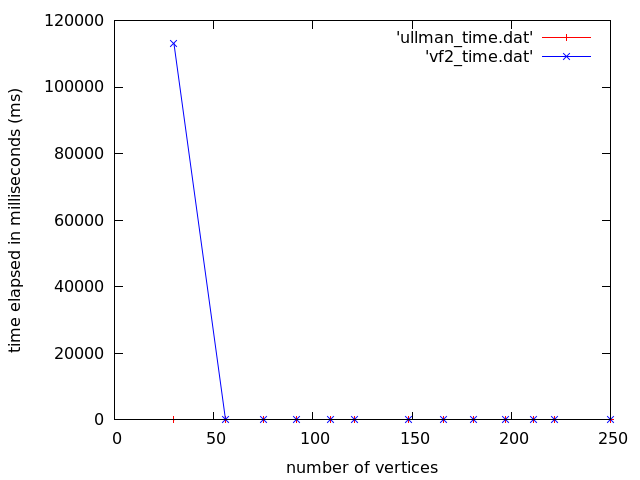
\includegraphics[width=0.8\textwidth]{time_comparison.png}
  \end{center}    
  \caption{Graph depiting the results for the time comparison between the algorithms for a set of joined graphs}
  \label{fig:time_comparison}
\end{figure}

\paragraph{Analysis of results}\mbox{}\\
Figure \ref{fig:time_comparison} depicts the comparison of the Ullman and the VF2 algorithms on the criteria of the time taken during the execution of the graph matching processes
of the respective algorithms.\newline\newline
The amount of time taken by the Ullman algorithm is depicted by the \textit{blue} line in figure \ref{fig:time_comparison}, and the time taken by VF2 algorithm 
is depicted by VF2 algorithm is depicted by the \textit{red} line in figure \ref{fig:time_comparison}.\newline\newline
Figure \ref{fig:time_comparison} depicts that the amount of time taken by the Ullman algorithm to successfully complete its graph matching processes is very 
small and consistant for the data set used in the experimentation.\newline\newline
The time taken by the VF2 algorithm however is very high for small sets of vertices, approximately \textit{40 - 60} vertices. But as the number of vertices 
increase, the amount of time declines rapidly and it equal to that of the Ullman algorithm.

\paragraph{Conclusion}\mbox{}\\
Based of figure \ref{fig:time_comparison}, it can be deduced that the time efficiency of the Ullman and VF2 algorithms are approximately equal to each other overall,
with the exception that for small graphs, the Ullman algorithm is more efficient than the VF2 algorithm in terms of the time taken to complete the graph matching
procedures.

\subsection{Empty graph results for the evaluation of different vertice numbers experiment}
This section presents the time and memory results for experiment described in section \ref{Performance evaluation for different vertice numbers}. The 
experiment is conducted on empty graphs.
\subsubsection{Memory Results}
This section depicts the memory results for the two algorithms on a set empty graphs of various vertice numbers. The red line depics the amount of memory
 used by the Ullman algorithm and the blue line depicts the amount of memory used by the VF2 algorithm.
\begin{figure}[H]
  \begin{center}
      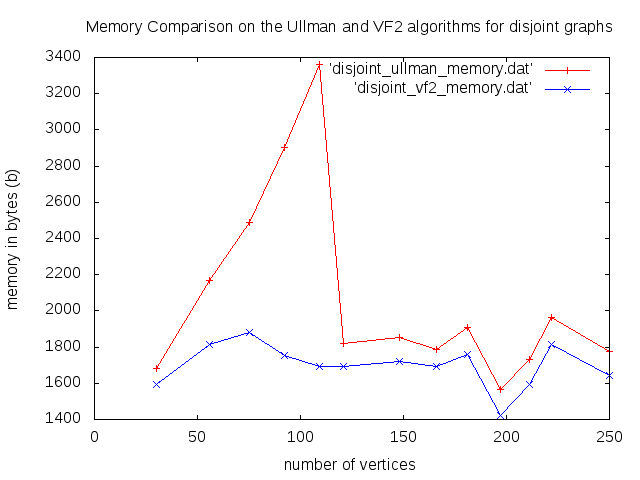
\includegraphics[width=0.8\textwidth]{disjoint_memory.png}
  \end{center}    
  \caption{Graph depiting the results for the memory comparison between the algorithms for a set of empty graphs}
  \label{fig:disjoint_memory_comparison}
\end{figure}

\paragraph{Analysis of results}\mbox{}\\
Figure \ref{fig:disjoint_memory_comparison} depicts the memory used by the two graphs by the two algorithms for a set of disjoint graphs with different vertice 
numbers.\newline\newline
The behavour of the two graphs appear to be very different for small graphs .i.e that is graphs with a size less than 120 approximately. The Ullman algorithm's
memory usage has a steep positive gradient from the beginning, and the gradient does not flactuate alot and stays consistant until it reaches its peeck.
The VF2 algorithm however does not have very steep gradient, and it reaches its peek faster than the Ullman algorithm.\newline\newline
The behavour of the algorithms is approximately similar, they both increase and crease and decrease their gradient in a similar pattern, even though the Ullman
 still uses a greater amount of memory than the VF2 algorithm.
 
\paragraph{Conclusion}\mbox{}\\
Based on figure \ref{fig:disjoint_memory_comparison}, it is clear that the VF2 more memory efficient than the Ullman algorithm. The its difference in memory 
usage is more vast for small disjoint graphs, and the Ullman algorithms demand for memory is very high and consistant. The algorithms have a similar 
performance for larger graphs, but the Ullman algorithm still has a larger demand of memory than the VF2 algorithm.


\subsubsection{Time Results}
This section reports the time taken by the algorithms to complete the graph matching procedure for a set of disjoint graphs with different number of vertices.The red line depics the amount of memory
 used by the Ullman algorithm and the blue line depicts the amount of memory used by the VF2 algorithm.

\begin{figure}[H]
  \begin{center}
      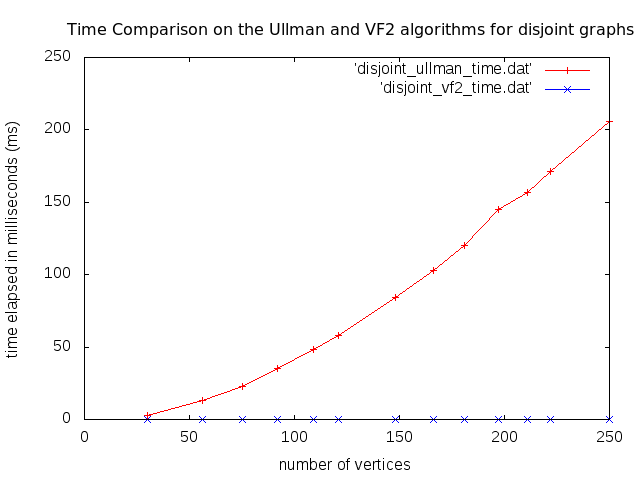
\includegraphics[width=0.8\textwidth]{disjoint_time.png}
  \end{center}    
  \caption{Graph depiting the results for the time comparison between the algorithms for a set of empty graphs}
  \label{fig:disjoint_time_comparison}
\end{figure}


\paragraph{Analysis of results}\mbox{}\\
 Figure \ref{fig:disjoint_time_comparison} depitcs the behavour of the two algorithms with regards to the amount of time taken by each algorithm to complete its 
 respective graph matching procedures.\newline\newline
 The Ullman algorithm has a gradually increasing slope that appears to be arbitrarily consistant throughout all the graph sizes. The VF2 algorithm has a 
 very constant and consistent behavour with regards to the time that it requires. The amount of time required seems to be neglibable for this algorithm as
  it seems to be very close to zero for all graph sizes.
  
 
  \newpage
\subimport{cases/}{cases}
  \newpage